\documentclass{beamer}
\usepackage{amsmath}
\usepackage{amssymb}
\usepackage{graphicx}
\usepackage[margin=1in]{geometry}
\newcommand{\del}{\nabla}
\begin{document}
\title{Extremal Optimization}
\author{Howon Lee}
\maketitle

\begin{frame}
  \frametitle{What is the question?}
  How can you use extremal dynamics to train some kind of neural net?
\end{frame}

\begin{frame}
  \frametitle{What? What's that?}
  Qualitative model of evolution: Bak-Sneppen model.
  \begin{figure}
    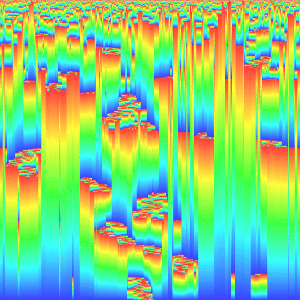
\includegraphics{bak_sneppen}
  \end{figure}

  Rules of Bak-Sneppen model. How does it behave?

  Caveats: CR Shalizi, W Tozier, "A Simple Model of the Evolution of Simple Models of Evolution"
\end{frame}

\begin{frame}
  \frametitle{Approaches Taken}
  Bak and Chialvo's model
  More abstract: extremal optimization
  Finally: Using $\tau$-EO on RBM
\end{frame}

\begin{frame}
  \frametitle{Adaptive Learning by Extremal Dynamics and Negative Feedback}
  %%% Bak and Chialvo do adaptive extremal optimization on a fake-ish neural net model. Conjunctive model means that it just sucks for problems like the parity problem, although the forgiveness thing ties everything together.
  How it works, from 20000 feet
  Problems: Conjunctive neurons
  Similarity to Tabu search, simulated annealing?
  %%% have my replication, and my results?
\end{frame}

\begin{frame}
  \frametitle{Results with Bak-Chialvo net}
  %%%% miserable results
  %%% shit results on Bak net. note that the shit results are a little less worse for natural data
\end{frame}

\begin{frame}
  \frametitle{More abstractly: EO, $\tau$-EO}
  How it works, from 20000 feet
  Existing results, from Boetticher: TSP
  %%% steal a chart
  %%% Talk about extremal optimization in the more abstract sense. Travelling salesman problem. Boetticher's work on the deterministic EO and tau-EO.
\end{frame}

\begin{frame}
  \frametitle{$\tau$-EO on neural nets}
  Why not feedforward?
  %%%% miserable results
\end{frame}


\begin{frame}
  \frametitle{Task}
  %%details of approach. specific target phenomenon. model network task setting, architecture, processing and learning algorithm, training environment
  %%% Figuring out applying the abstract EO algorithm to things. Note that the locality of fitness that the model requires is much easier to do in Boltzmann machine, decide to do RBM on those machines.
\end{frame}

\begin{frame}
  \frametitle{Results on RBM}
  %%%% charts charts charts
  %%% Results. Try some classifications. Do time course of learning on the shit error measure that we have and a non-shit error measure. Compare to gradient descent for learning. Apologize for not having simulated annealing to compare to.
\end{frame}

\begin{frame}
  \frametitle{Problems, Issues}
  %%%% presumably I have some problems and issues

\end{frame}

\begin{frame}
  \frametitle{Going forward}
  In report: compare with simulated annealing
  In report: look at created weights
  After class: use in a deep architecture
  After class: investigate with non-restricted BM's
  %%%% speculation speculation speculation
\end{frame}

\end{document}

